%
% Although we try to provide a template that completely
% matches the corresponding assignment, we do expect you
% to check that you have indeed answered all questions.
%

% ALSO VERY IMPORTANT:
% This is just a template to help you with the LaTeX part of the assignment.
% So you may change it completely according to your own wishes!
%

\documentclass[a4paper]{article}
% Typically the 'article' class is appropriate for assignments.
% And we print it on a4, so we include that as well.

\usepackage{a4wide}
% To decrease the margins and allow more text on a page.

\usepackage{graphicx}
% To deal with including pictures.

\usepackage{enumerate}
% To provide a little bit more functionality than with LaTeX's default
% enumerate environment.

\usepackage{array}
% To provide a little bit more functionality than with LaTeX's default
% array environment.

\usepackage[american]{babel}
% Use this if you want to write the document in US English. It takes care of
% (usually) proper hyphenation.
% If you want to write your answers in Dutch, please replace 'american'
% by 'dutch'.
% Note that after a change it may be that the first compilation of LaTeX
% fails. That is normal and caused by the fact that in auxiliary files
% from previous runs, there may still be a \selectlanguage{american}
% around, which is invalid if 'american' is not incorporated with babel.

\usepackage{amssymb}
% This package loads mathematical things like the fonts for the blackboard
% bold for the set of natural numbers.
\usepackage{amsmath}
% And some student asked me to include amsmath as well...

\usepackage{tikz}
\usetikzlibrary{arrows}
\usetikzlibrary{positioning}
% The tikz package can be used to draw all kinds of diagrams.
% In this assignment it is being used for drawing the parse trees


\usepackage{xspace}
% xspace can be used to let LaTeX decide whether a command should be followed
% y a space or not, depending on what follows.

% Some obscure definition to create a circled node within xy.
% The definition is made by Freek Wiedijk who prefers to do his definitions
% in TeX instead of LaTeX, which explains the \def instead of \newcommand.
\def\node{*++[o][F-]}
\def\fnode{*++[o][F=]}

\usepackage{csquotes}
\usepackage{mathtools}

% This command puts a `def' on top of an `='.
\newcommand{\isdef}{\ensuremath{\,\,\buildrel\rm def\over=}\,\,}

\reversemarginpar
\title{Linear Algebra for AI\\Assignment 4}

\author{Tony Lopar \\ s1013792 \\ Group 5 \quad Felicity Reddel}

\begin{document}
\maketitle

\section*{Exercise 1}
% (i) F : R3 → R3 defined by F(x, y, z) = (x − y + 2z, 3x + y − z, 4x + z).
\begin{enumerate}[i)]
  \item In order to find the dimension for the kernel and image of F we may put the mappings in s matrix and try to find the number of basic solutions.
  \[
  \left(
  \begin{array}{ccc}
  1 & -1 & 2 \\
  3 & 1 & -1 \\
  4 & 0 & 1 \\
  \end{array}
  \right)
  \xrightarrow{\text{$R_2 := R_2 + 1 \cdot R_1$}}
    \left(
    \begin{array}{ccc}
    1 & -1 & 2 \\
    4 & 0 & 1 \\
    4 & 0 & 1 \\
    \end{array}
    \right)
    \xrightarrow{\text{$R_3 := R_3 + (-1) \cdot R_2$}}
      \left(
      \begin{array}{ccc}
      1 & -1 & 2 \\
      4 & 0 & 1 \\
      0 & 0 & 0 \\
      \end{array}
      \right)
  \]
  \[
  \xrightarrow{\text{$R_2 := R_2 + (-4) \cdot R_1$}}
    \left(
    \begin{array}{ccc}
    1 & -1 & 2 \\
    0 & 4 & -7 \\
    0 & 0 & 0 \\
    \end{array}
    \right)
    \xrightarrow{\text{$R_2 := \frac{1}{4} \cdot R_2$}}
      \left(
      \begin{array}{ccc}
      1 & -1 & 2 \\
      0 & 1 & - \frac{7}{4} \\
      0 & 0 & 0 \\
      \end{array}
      \right)
      \xrightarrow{\text{$R_1 := R_1 + 1 \cdot R_2$}}
        \left(
        \begin{array}{ccc}
        1 & 0 & \frac{1}{4} \\
        0 & 1 & - \frac{7}{4} \\
        0 & 0 & 0 \\
        \end{array}
        \right)
  \]
  From the matrix in reduced Echelon form we may see that the dimension of the image is 2, since there are two pivots. Furthermore, we see that the dimenstion of the kernel is 1, since there is only one column without pivot. Finally, we see that (x, y, z) is only in the kernel if and only if:
  \begin{align*}
    x + \frac{1}{4} z &= 0 \\
    x &= - \frac{1}{4} z \\
    y - \frac{7}{4} z &= 0 \\
    y &= \frac{7}{4} z
  \end{align*}
  So the kernel of F consists of all vectors in the form $(-\frac{1}{4}z, \frac{7}{4}z, z)$ which is equivalent to all scalar multiples of $(-1, 7, 4)$. This shows that the following vector is a basis for the kernel of F:
  \[
  \left(
  \begin{array}{c}
  -1 \\
  7 \\
  4 \\
  \end{array}
  \right)
  \]
  \item We may put this mappings in a matrix either and transform this to (reduced) Echelon form to find the dimensions.
  % (ii) F : R3 → R4 defined by F(x, y, z) = (−x + 2y + 3z, x + y, 3y + 3z, x + 7y + 6z).
  \[
  \left(
  \begin{array}{ccc}
  -1 & 2 & 3 \\
  1 & 1 & 0 \\
  0 & 3 & 3 \\
  1 & 7 & 6 \\
  \end{array}
  \right)
  \xrightarrow{\text{$R_1 := R_1 + 1 \cdot R_2$}}
  \left(
  \begin{array}{ccc}
  0 & 3 & 3 \\
  1 & 1 & 0 \\
  0 & 3 & 3 \\
  1 & 7 & 6 \\
  \end{array}
  \right)
  \xrightarrow{\text{$R_1 \leftrightarrow R_4$}}
  \left(
  \begin{array}{ccc}
  1 & 7 & 6 \\
  1 & 1 & 0 \\
  0 & 3 & 3 \\
  0 & 3 & 3 \\
  \end{array}
  \right)
  \]
  \[
  \xrightarrow{\text{$R_1 := R_1 + (-2) \cdot R_3$}}
  \left(
  \begin{array}{ccc}
  1 & 1 & 0 \\
  1 & 1 & 0 \\
  0 & 3 & 3 \\
  0 & 3 & 3 \\
  \end{array}
  \right)
  \xrightarrow{\text{$R_4 := R_4 + (-1) \cdot R_3$}}
  \left(
  \begin{array}{ccc}
  1 & 1 & 0 \\
  1 & 1 & 0 \\
  0 & 3 & 3 \\
  0 & 0 & 0 \\
  \end{array}
  \right)
  \]
  \[
  \xrightarrow{\text{$R_2 := R_2 + (-1) \cdot R_1$}}
  \left(
  \begin{array}{ccc}
  1 & 1 & 0 \\
  0 & 0 & 0 \\
  0 & 3 & 3 \\
  0 & 0 & 0 \\
  \end{array}
  \right)
  \xrightarrow{\text{$R_2 \leftrightarrow R_3$}}
  \left(
  \begin{array}{ccc}
  1 & 1 & 0 \\
  0 & 3 & 3 \\
  0 & 0 & 0 \\
  0 & 0 & 0 \\
  \end{array}
  \right)
  \]
  \[
  \xrightarrow{\text{$R_2 := \frac{1}{3} \cdot R_2$}}
  \left(
  \begin{array}{ccc}
  1 & 1 & 0 \\
  0 & 1 & 1 \\
  0 & 0 & 0 \\
  0 & 0 & 0 \\
  \end{array}
  \right)
  \xrightarrow{\text{$R_1 := R_1 + (-1) \cdot R_2$}}
  \left(
  \begin{array}{ccc}
  1 & 0 & -1 \\
  0 & 1 & 1 \\
  0 & 0 & 0 \\
  0 & 0 & 0 \\
  \end{array}
  \right)
  \]
  In the reduced Echelon form of the matrix we see that the dimension of the image is 2, since there are two pivot columns in the matrix. Furthermore, we see that the dimension of the kernel is 1, since there is only one non-pivot column. Finally, we see that (x, y, z) is only in the kernel if and only if:
  \begin{align*}
    x - z &= 0 \\
    x &= z \\
    y + z &= 0 \\
    y &= -z
  \end{align*}
  So the kernel of F consists of all vectors in the form $(z, -z, z)$ which is equivalent to all scalar multiples of $(1, -1, 1)$. This shows that the following vector is a basis for the kernel of F:
  \[
  \left(
  \begin{array}{c}
  1 \\
  -1 \\
  1 \\
  \end{array}
  \right)
  \]
\end{enumerate}

\section*{Exercise 2}
This network can be represented in the graph of figure~\ref{fig:M1}. I put the nodes in this form to prevent edges from crossing.
\begin{figure}[h]
\begin{center}
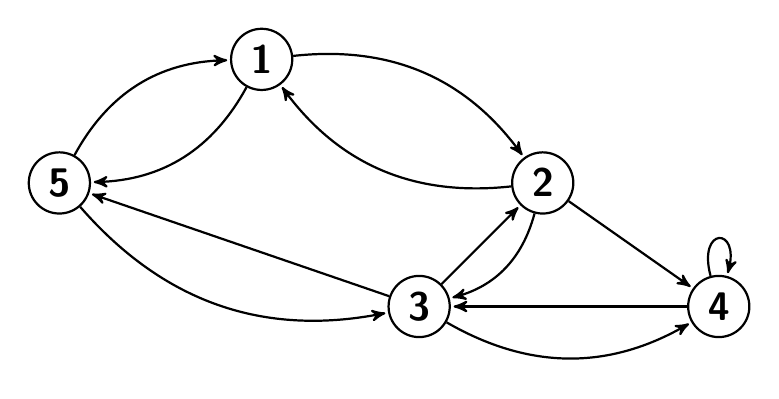
\begin{tikzpicture}[->,>=stealth',shorten >=1pt,auto,node distance=2cm, every loop/.style={},
                    thick, ,main node/.style={circle,draw,font=\sffamily\Large\bfseries}]

  \node[main node] (1) {1};
  \node[main node] (2) [below right=1cm and 3cm of 1] {2};
  \node[main node] (3) [below left=1cm and 1cm of 2] {3};
  \node[main node] (5) [below left=1cm and 2cm of 1] {5};
  \node[main node] (4) [right=1cm and 3cm of 3] {4};

  \path[every node/.style={font=\sffamily\normalsize, text = black }]
    (1) edge[bend left] node [left] {} (2)
        edge[bend left] node [left] {} (5)
    (2) edge[bend left] node [left] {} (1)
        edge[bend left] node [left] {} (3)
        edge[left] node [left] {} (4)
    (3) edge[left] node [left] {} (2)
        edge[bend right] node [left] {} (4)
        edge[left] node [left] {} (5)
    (4) edge[right] node [left] {} (3)
        edge[loop above] node [left] {} ()
    (5) edge[bend left] node [left] {} (1)
        edge[bend right] node [left] {} (3)
    ;
\end{tikzpicture}
\caption{Graphical representation} \label{fig:M1}
\end{center}
\end{figure}

In order to get the two step path we should multiply the matrix of the network with itself. This will result in the $A^2$ matrix which shows the number of possible 2-step paths.
\begin{align*}
\left(
\begin{array}{ccccc}
0 & 1 & 0 & 0 & 1 \\
1 & 0 & 1 & 1 & 0 \\
0 & 1 & 0 & 1 & 1 \\
0 & 0 & 1 & 1 & 0 \\
1 & 0 & 1 & 0 & 0 \\
\end{array}
\right)
\cdot
\left(
\begin{array}{ccccc}
0 & 1 & 0 & 0 & 1 \\
1 & 0 & 1 & 1 & 0 \\
0 & 1 & 0 & 1 & 1 \\
0 & 0 & 1 & 1 & 0 \\
1 & 0 & 1 & 0 & 0 \\
\end{array}
\right)
&=
\left(
\begin{array}{ccccc}
2 & 0 & 2 & 1 & 0 \\
0 & 2 & 1 & 2 & 2 \\
2 & 0 & 3 & 2 & 0 \\
0 & 1 & 1 & 2 & 1 \\
0 & 2 & 0 & 1 & 2 \\
\end{array}
\right)
\end{align*}

In order to find the paths with a length of exactly three from 2 to 3 we should use the matrix calculated for paths of length two. We should pick from this the row of point 2 and multiply this with the column of point 3 in the array of paths with length one. So, This will give us the value for the number of paths.
\[
\left(
\begin{array}{ccccc}
0 & 2 & 1 & 2 & 2 \\
\end{array}
\right)
\cdot
\left(
\begin{array}{c}
0 \\
1 \\
0 \\
1 \\
1 \\
\end{array}
\right)
=
0 \cdot 0 + 2 \cdot 1 + 1 \cdot 0 + 2 \cdot 1 + 2 \cdot 1 = 6
\]

% f(x1, x2, x3) = (x1 − 2x2, x2 + 2x3) and g(y1, y2) =(y1 − 2y2, 3y2)
\section*{Exercise 3}
\begin{enumerate}
  \item We can construct the composite function $g \circ f$ as follows:
  \begin{align*}
    (g \circ f)(x_1, x_2, x_3)  &= g(f(x_1, x_2, x_3)) \\
                                &= g(x_1 - 2x_2, x_2 + 2x_3) \\
                                &= ((x_1 - 2x_2) - 2(x_2 + 2x_3), 3(x_2 + 2x_3)) \\
                                &= (x_1 - 2x_2 - 2x_2 - 4x_3, 3x_2 + 6x_3)) \\
                                &= (x_1 - 4x_2 - 4x_3, 3x_2 + 6x_3))
  \end{align*}
  This composition leads to the following matrix:
  \[
  \left(
  \begin{array}{ccc}
  1 & -4 & -4 \\
  0 & 3 & 6 \\
  \end{array}
  \right)
  \]
  \item We matrices for the functions g and f are as follows:
  \[
  M_g =
  \left(
  \begin{array}{cc}
  1 & -2 \\
  0 & 3 \\
  \end{array}
  \right)
  \enspace
  M_f =
  \left(
  \begin{array}{ccc}
  1 & -2 & 0 \\
  0 & 1 & 2 \\
  \end{array}
  \right)
  \]
  We can calculate $M_{g \circ f}$ by multiplying the matrix $M_g$ with $M_f$. This results in the following matrix:
  \[
  \left(
  \begin{array}{cc}
  1 & -2 \\
  0 & 3 \\
  \end{array}
  \right)
  \cdot
  \left(
  \begin{array}{ccc}
  1 & -2 & 0 \\
  0 & 1 & 2 \\
  \end{array}
  \right)
  =
  \left(
  \begin{array}{ccc}
  1 \cdot 1 + 0 \cdot 0 & 1 \cdot - 2 + - 2 \cdot 1 & 1 \cdot 0 + - 2 \cdot 2  \\
  0 \cdot 1 + 3 \cdot 0 & 0 \cdot - 2 + 3 \cdot 1 & 0 \cdot 0 + 3 \cdot 2  \\
  \end{array}
  \right)
  =
  \left(
  \begin{array}{ccc}
  1 & -4 & -4 \\
  0 & 3 & 6 \\
  \end{array}
  \right)
  \]
\end{enumerate}

\section*{Exercise 4}
I constructed the transition matrix by first filling in the percentage of people that stay at the insurance company. These values are on the diagonal. After this I filled in the values for the people for which the switch is defined in the assignment. We see that $10 \%$ of the customers switch from A to C, so we fill this in the cell which represents from A to C. This is the cell in the first column and the third row. We also do this for the other transitions. Since the numbers don't correspond for all customers since the percentages don't reach the $100 \%$ I put the remaining percentage in the transition that's undefined. So for example, the transition from A to B becomes $10 \%$, since only $90 \%$ remains at a or takes the transition to C. We see that for all of the three companies only the transition of $90 \%$ of the customers is defined, so we should add $10 \%$ to the empty cells. This gives the following transition matrix:
\[
\left(
\begin{array}{ccc}
0.8 & 0.2 & 0.3 \\
0.1 & 0.7 & 0.1 \\
0.1 & 0.1 & 0.6 \\
\end{array}
\right)
\]
In order to compute the distribution in one year we can multiply the values with the values for the current distribution. We see that the distribution for company B isn't specified, so we can compute this as $100 \% - 60 \% - 30 \% = 10 \%$.
\[
\left(
\begin{array}{ccc}
0.8 & 0.2 & 0.3 \\
0.1 & 0.7 & 0.1 \\
0.1 & 0.1 & 0.6 \\
\end{array}
\right)
\cdot
\left(
\begin{array}{ccc}
0.3 \\
0.1 \\
0.6 \\
\end{array}
\right)
=
\left(
\begin{array}{c}
0.8 \cdot 0.3 + 0.2 \cdot 0.1 + 0.3 \cdot 0.6 \\
0.1 \cdot 0.3 + 0.7 \cdot 0.1 + 0.1 \cdot 0.6 \\
0.1 \cdot 0.3 + 0.1 \cdot 0.1 + 0.6 \cdot 0.6 \\
\end{array}
\right)
=
\left(
\begin{array}{c}
0.44 \\
0.16 \\
0.4 \\
\end{array}
\right)
\]
We see that after one year $44 \%$ is customer of company A, $16 \%$ of company B and $40 \%$ of company C.

In order to compute the probability that we stay with company C we should multiply the row with to C two times with the column from C.
\[
\left(
\begin{array}{ccc}
0.1 & 0.1 & 0.6 \\
\end{array}
\right)
\cdot
\left(
\begin{array}{c}
0.3 \\
0.1 \\
0.6 \\
\end{array}
\right)
=
(0.1 \cdot 0.3 + 0.1 \cdot 0.1 + 0.6 \cdot 0.6) = 0.4
\]
We see that the probability that we end up in C after two years is $40 \%$.
% , so the change the we remain at company C after two years is $0.4^2 = 16 \%$.
\end{document}
